\section{interpreter.c File Reference}
\label{interpreter_8c}\index{interpreter.c@{interpreter.c}}
{\tt \#include $<$string.h$>$}\par
{\tt \#include $<$stdio.h$>$}\par
{\tt \#include $<$stdlib.h$>$}\par
{\tt \#include \char`\"{}ueac.h\char`\"{}}\par
{\tt \#include \char`\"{}interpreter.h\char`\"{}}\par
{\tt \#include \char`\"{}ueaclib.h\char`\"{}}\par
{\tt \#include \char`\"{}calibrate.h\char`\"{}}\par


Include dependency graph for interpreter.c:\begin{figure}[H]
\begin{center}
\leavevmode
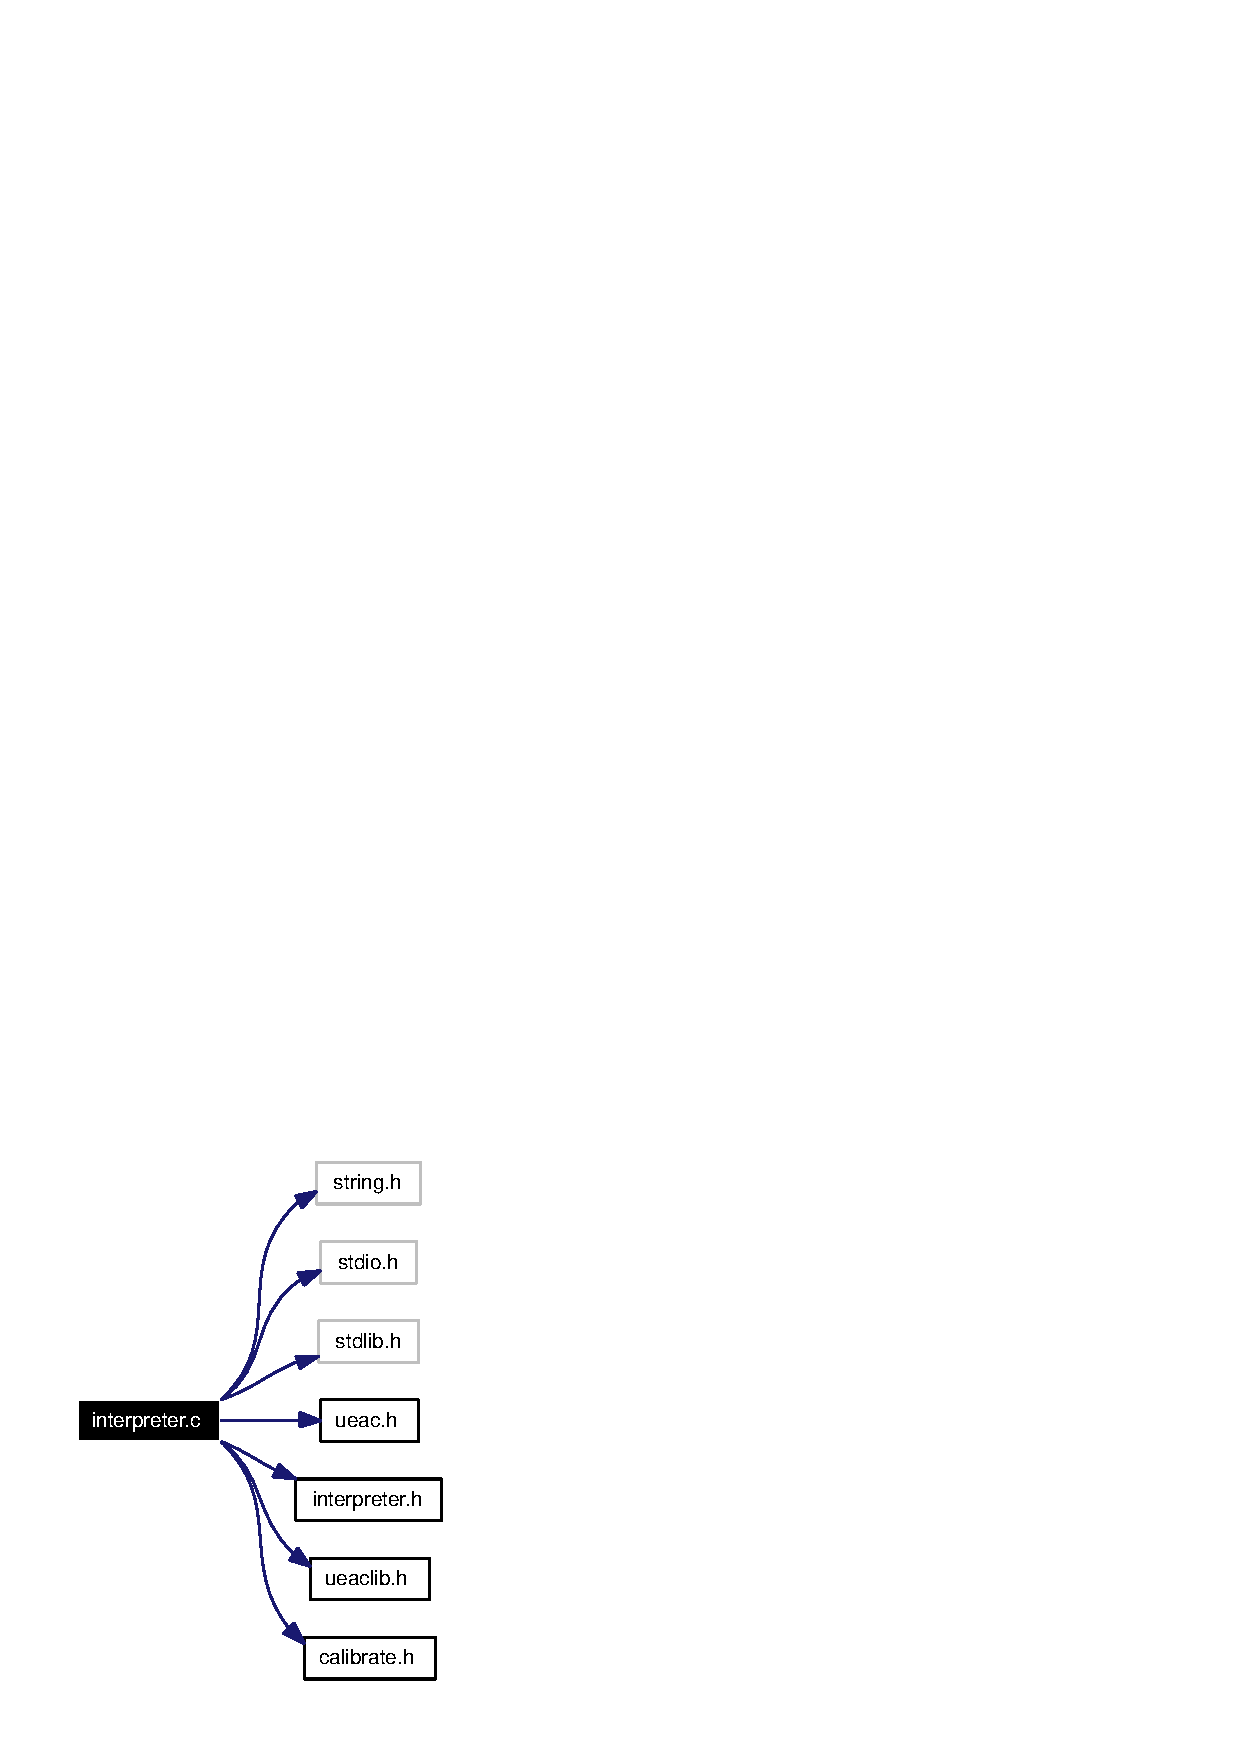
\includegraphics[width=106pt]{interpreter_8c__incl}
\end{center}
\end{figure}
\subsection*{Functions}
\begin{CompactItemize}
\item 
int {\bf delspace} (char $\ast$instr, char $\ast$outstr)
\item 
int {\bf interpreter} (char $\ast$command\_\-string, {\bf ueac\_\-t} $\ast$system\_\-state)
\end{CompactItemize}
\subsection*{Variables}
\begin{CompactItemize}
\item 
const char {\bf DELIMITER} [$\,$] = \char`\"{},\char`\"{}
\item 
const char {\bf TERMINATOR} [$\,$] = \char`\"{}$\backslash$n\char`\"{}
\item 
const char {\bf RST} [$\,$] = \char`\"{}RST$\backslash$n\char`\"{}
\item 
const char {\bf CAL} [$\,$] = \char`\"{}CAL$\backslash$n\char`\"{}
\item 
const char {\bf LON} [$\,$] = \char`\"{}LON$\backslash$n\char`\"{}
\item 
const char {\bf LOF} [$\,$] = \char`\"{}LOF$\backslash$n\char`\"{}
\item 
const char {\bf GRID\_\-NUM\_\-MIN} [$\,$] = \char`\"{}1\char`\"{}
\item 
const char {\bf GRID\_\-NUM\_\-MAX} [$\,$] = \char`\"{}5\char`\"{}
\end{CompactItemize}


\subsection{Function Documentation}
\index{interpreter.c@{interpreter.c}!delspace@{delspace}}
\index{delspace@{delspace}!interpreter.c@{interpreter.c}}
\subsubsection{\setlength{\rightskip}{0pt plus 5cm}int delspace (char $\ast$ {\em instr}, char $\ast$ {\em outstr})}\label{interpreter_8c_a8}




Definition at line 66 of file interpreter.c.

Referenced by interpreter().

\footnotesize\begin{verbatim}66                                        {
67   int length=0;
68   while (*instr!='\0') {
69     if (*instr!=' ') {
70       *outstr=*instr;
71       outstr++;
72       length++;
73     }
74     instr++;
75   }
76   *outstr='\0';
77   return length;
78 }
\end{verbatim}\normalsize 


\index{interpreter.c@{interpreter.c}!interpreter@{interpreter}}
\index{interpreter@{interpreter}!interpreter.c@{interpreter.c}}
\subsubsection{\setlength{\rightskip}{0pt plus 5cm}int interpreter (char $\ast$ {\em command\_\-string}, {\bf ueac\_\-t} $\ast$ {\em system\_\-state})}\label{interpreter_8c_a9}




Definition at line 81 of file interpreter.c.

References CAL, ueac\_\-instruction::command\_\-reg, DELIMITER, delspace(), ueac::instruction, ueac\_\-instruction::instruction\_\-type, ueac\_\-instruction::lla\_\-descriptor, ueac\_\-instruction::lla\_\-function, ueac\_\-instruction::lla\_\-period, LOF, LON, ueac\_\-instruction::pin\_\-x, ueac\_\-instruction::pin\_\-x\_\-alt, ueac\_\-instruction::pin\_\-y, ueac\_\-instruction::pin\_\-y\_\-alt, RST, TERMINATOR, UEAC\_\-ALL\_\-I, UEAC\_\-ALL\_\-V, UEAC\_\-CAL, UEAC\_\-EXECUTE, ueac\_\-execute\_\-instruction(), UEAC\_\-LLA\_\-ADD, UEAC\_\-LLA\_\-DISABLE, UEAC\_\-LLA\_\-ENABLE, UEAC\_\-LLA\_\-REPORT, UEAC\_\-LOF, UEAC\_\-LON, UEAC\_\-READ\_\-I, UEAC\_\-READ\_\-V, UEAC\_\-RST, UEAC\_\-WRITE, ueac\_\-instruction::value, W\_\-VALUE\_\-MAX, and W\_\-VALUE\_\-MIN.

Referenced by main().

\footnotesize\begin{verbatim}81                                                             {
82   enum {COMMAND,SPECIFIER,F3,F4,F5,F6,F7,F8,F9,F10};           // field states
83   enum {R_PRIMITIVE,W_PRIMITIVE,PRINTGRID,LLA,GLOBAL_CONTROL};  // instruction type
84   enum {NOT_DONE,DONE,FAILED};
85 
86   char *token = NULL;
87   unsigned char error_code = 0;
88   int field = COMMAND;                                    // State variable to indicated which delimited 
89   int type = R_PRIMITIVE;                                 // State varible to indicate the context of the field
90   char *strptr=NULL;
91   char tokbuf[20];                                        // field buffer used to strip spaces from the input
92   int command_complete = NOT_DONE;                        // Variable to indicate if the command string has an issue 
93   char *tokend;
94   long result_temp;
95 
96   while (system_state->instruction.command_reg==UEAC_EXECUTE); // wait while the last command completes
97   token = strtok(command_string,DELIMITER);                    // grab the next token and pass it to the field parser  
98   while ((token!=NULL)&&(command_complete!=FAILED)) {          // stop when strtok returns NULL or parsing fails
99     delspace(token,tokbuf);
100     switch (field) {
101     // Parse the individual fields
102     case COMMAND:   
103       if (!strcasecmp(tokbuf,"R")) {
104         type = R_PRIMITIVE;
105       }
106       else if (!strcasecmp(tokbuf,"W")) {
107         type = W_PRIMITIVE;
108       }
109       else if (!strcasecmp(tokbuf,"P")) {
110         type = PRINTGRID;
111       }
112       else if (!strcasecmp(tokbuf,"L")) {
113         type = LLA;
114       }
115       else if (!strcasecmp(tokbuf,RST)) {
116         system_state->instruction.instruction_type=UEAC_RST;
117         command_complete=DONE;
118       }
119       else if (!strcasecmp(tokbuf,CAL)) {
120         system_state->instruction.instruction_type=UEAC_CAL;
121         command_complete=DONE;
122       }
123       else if (!strcasecmp(tokbuf,LON)) {
124         system_state->instruction.instruction_type=UEAC_LON;
125         command_complete=DONE;
126       }
127       else if (!strcasecmp(tokbuf,LOF)) {
128         system_state->instruction.instruction_type=UEAC_LOF;
129         command_complete=DONE;
130       }
131       else {
132         command_complete=FAILED;
133         error_code=1;
134       }
135       field=SPECIFIER;
136       break;
137     case SPECIFIER:
138       switch (type) {
139         // Parse field based on specifics of the particular command type
140       case R_PRIMITIVE:
141         if (!strcasecmp(tokbuf,"V")) {
142           system_state->instruction.instruction_type=UEAC_READ_V;
143           field = F3;
144         }
145         else if (!strcasecmp(tokbuf,"I")) {
146           system_state->instruction.instruction_type=UEAC_READ_I;
147           field = F3;
148         }
149         else {
150           command_complete=FAILED;
151           error_code=2;
152         }
153         break;
154       case W_PRIMITIVE:
155         if (!strcasecmp(tokbuf,"I")) {
156           system_state->instruction.instruction_type=UEAC_WRITE;
157           field = F3;
158         }
159         else {
160           command_complete=FAILED;
161           error_code=3;
162         }
163         break;
164       case PRINTGRID:
165         if ((strptr=strchr(tokbuf,'\n'))==NULL) {
166           // newline not found which is an error in this field. 
167           command_complete=FAILED;
168           error_code=4;
169           break;
170         }
171         else {
172           *strptr=0; // since newline found, strip it from tokbuf for V/I match
173         }
174         // Parse the field now that the newline has been located
175         if (!strcasecmp(tokbuf,"V")) {
176           system_state->instruction.instruction_type=UEAC_ALL_V;
177           command_complete=DONE;
178         }
179         else if (!strcasecmp(tokbuf,"I")) {
180           system_state->instruction.instruction_type=UEAC_ALL_I;
181           command_complete=DONE;
182         }
183         else {
184          command_complete=FAILED;
185          error_code=5;
186         }
187         break;
188       case LLA:
189         if (!strcasecmp(tokbuf,"A")) {
190           system_state->instruction.instruction_type=UEAC_LLA_ADD;
191           field = F3;
192         }
193         else if (!strcasecmp(tokbuf,"D")) {
194           system_state->instruction.instruction_type=UEAC_LLA_DISABLE;
195           field = F3;
196         }
197         else if (!strcasecmp(tokbuf,"E")) {
198           system_state->instruction.instruction_type=UEAC_LLA_ENABLE;
199           field = F3;
200         }
201         else if (!strcasecmp(tokbuf,"R")) {
202           system_state->instruction.instruction_type=UEAC_LLA_REPORT;
203           field = F3;
204         }
205         else {
206          command_complete=FAILED;
207          error_code=5;
208         }
209       }
210       break;
211     case F3:
212       switch (type) {
213       case R_PRIMITIVE:
214       case W_PRIMITIVE:  
215       case LLA:
216         // For RW/LLA this should be the X location (XIN)
217         result_temp=strtol(tokbuf,&tokend,10);
218         if (*tokend!=0) {
219           command_complete=FAILED;
220           error_code=6;
221         }
222         else {
223           if ((result_temp>=1)&&(result_temp<=5)) {
224             system_state->instruction.pin_x=(unsigned char) result_temp;
225             field=F4;
226           }
227           else {
228             command_complete=FAILED;
229             error_code=6;
230           }
231         }
232         break;
233       }
234       break;
235     case F4:
236       switch (type) {
237       case R_PRIMITIVE:
238       case W_PRIMITIVE:
239       case LLA:
240         // For RW/LLA this should be the Y location (LLA YIN)
241         result_temp=strtol(tokbuf,&tokend,10);
242         if (*tokend!=0) {
243           command_complete=FAILED;
244           error_code=6;
245         }
246         else {
247           if ((result_temp>=1)&&(result_temp<=5)) {
248             system_state->instruction.pin_y=(unsigned char) result_temp;
249             field=F5;
250           }
251           else {
252             command_complete=FAILED;
253             error_code=9;
254           }
255         }
256         break;
257       }
258       break;
259     case F5:
260       switch (type) {
261       case R_PRIMITIVE:
262       case W_PRIMITIVE:
263         // For RW this should be the value field
264         if ((strptr=strchr(tokbuf,'\n'))==NULL) {
265           command_complete=FAILED; // lack of newline is an error in this field. 
266           error_code=10;
267           break;
268         }
269         else {
270           *strptr=0; // since newline found, strip it from tokbuf for V/I match
271         }
272         result_temp=strtol(tokbuf,&tokend,10);
273         if (*tokend!=0) {
274           command_complete=FAILED;
275           error_code=6;
276         }
277         else {
278           if ((result_temp<=W_VALUE_MAX)&&(result_temp>=W_VALUE_MIN)) {
279             system_state->instruction.value=result_temp;
280             command_complete=DONE;
281           }
282           else {
283             command_complete=FAILED;
284             error_code=12;
285           }
286         }
287         break;
288       case LLA:
289         // For LLA this should be the X Output location
290         result_temp=strtol(tokbuf,&tokend,10);
291         if (*tokend!=0) {
292           command_complete=FAILED;
293           error_code=6;
294         }
295         else {
296           if ((result_temp>=0)&&(result_temp<=5)) {
297             system_state->instruction.pin_x_alt=(unsigned char) result_temp;
298             field=F6;
299           }
300           else {
301             command_complete=FAILED;
302             error_code=9;
303           }
304         }
305         break;
306       }
307       break;
308     case F6:
309       switch (type) {
310       case LLA:
311         // For LLA this should be the Y Output location
312         result_temp=strtol(tokbuf,&tokend,10);
313         if (*tokend!=0) {
314           command_complete=FAILED;
315           error_code=6;
316         }
317         else {
318           if ((result_temp>=0)&&(result_temp<=5)) {
319             system_state->instruction.pin_y_alt=(unsigned char) result_temp;
320             field=F7;
321           }
322           else {
323             command_complete=FAILED;
324             error_code=9;
325           }
326         }
327         break;
328       }
329       break;
330     case F7:
331       switch (type) {
332       case LLA:
333         // For LLA commands this is the numeric descriptor for the LLA
334         result_temp=strtol(tokbuf,&tokend,10);
335         if (*tokend!=0) {
336           command_complete=FAILED;
337           error_code=6;
338         }
339         else {
340           if ((result_temp>0)&&(result_temp<=10)) {
341             system_state->instruction.lla_descriptor=(unsigned char) result_temp;
342             field=F8;
343           }
344           else {
345             command_complete=FAILED;
346             error_code=6;
347           }
348         }
349         break;
350       }
351       break;
352     case F8:
353       switch (type) {
354       case LLA:
355         // For LLA commands this is the lla_function
356         result_temp=strtol(tokbuf,&tokend,10);
357         if (*tokend!=0) {
358           command_complete=FAILED;
359           error_code=6;
360         }
361         else {
362           if ((result_temp>0)&&(result_temp<=52)) {
363             system_state->instruction.lla_function=(unsigned char) result_temp;
364             field=F9;
365           }
366           else {
367             command_complete=FAILED;
368             error_code=6;
369           }
370         }
371         break;
372       }
373       break;
374     case F9:
375         // For LLA commands this is the lla_period
376       switch (type) {
377       case LLA:
378         // For LLA 
379         if ((strptr=strchr(tokbuf,'\n'))==NULL) {
380           command_complete=FAILED; // lack of newline is an error in this field. 
381           error_code=10;
382           break;
383         }
384         else {
385           *strptr=0; // since newline found, strip it from tokbuf for V/I match
386         }
387         result_temp=strtol(tokbuf,&tokend,10);
388         if (*tokend!=0) {
389           command_complete=FAILED;
390           error_code=6;
391         }
392         else {
393           if ((result_temp>0)&&(result_temp<=255)) {
394             system_state->instruction.lla_period=(unsigned char) result_temp;
395             command_complete=DONE;
396           }
397           else {
398             command_complete=FAILED;
399             error_code=6;
400           }
401         }
402         break;
403       }
404       break;
405     case F10:
406       if (!strncasecmp(tokbuf,TERMINATOR,sizeof(TERMINATOR))) {
407         printf("Found Terminator\n");
408       }
409       else {
410         printf("F10 %s\n",tokbuf);
411       }
412       break;
413     }
414     token = strtok(NULL,DELIMITER);  // get the next token 
415   }
416   if (command_complete==DONE) {
417     system_state->instruction.command_reg=UEAC_EXECUTE;
418     ueac_execute_instruction(system_state);
419     while (system_state->instruction.command_reg==UEAC_EXECUTE); // wait while the last command completes
420   }
421   else {
422 #ifndef LINUX 
423     printf("NOK\n\r");
424 #else
425     printf("NOK\n");
426 #endif 
427   }
428   return error_code;
429 }
\end{verbatim}\normalsize 




Here is the call graph for this function:\begin{figure}[H]
\begin{center}
\leavevmode
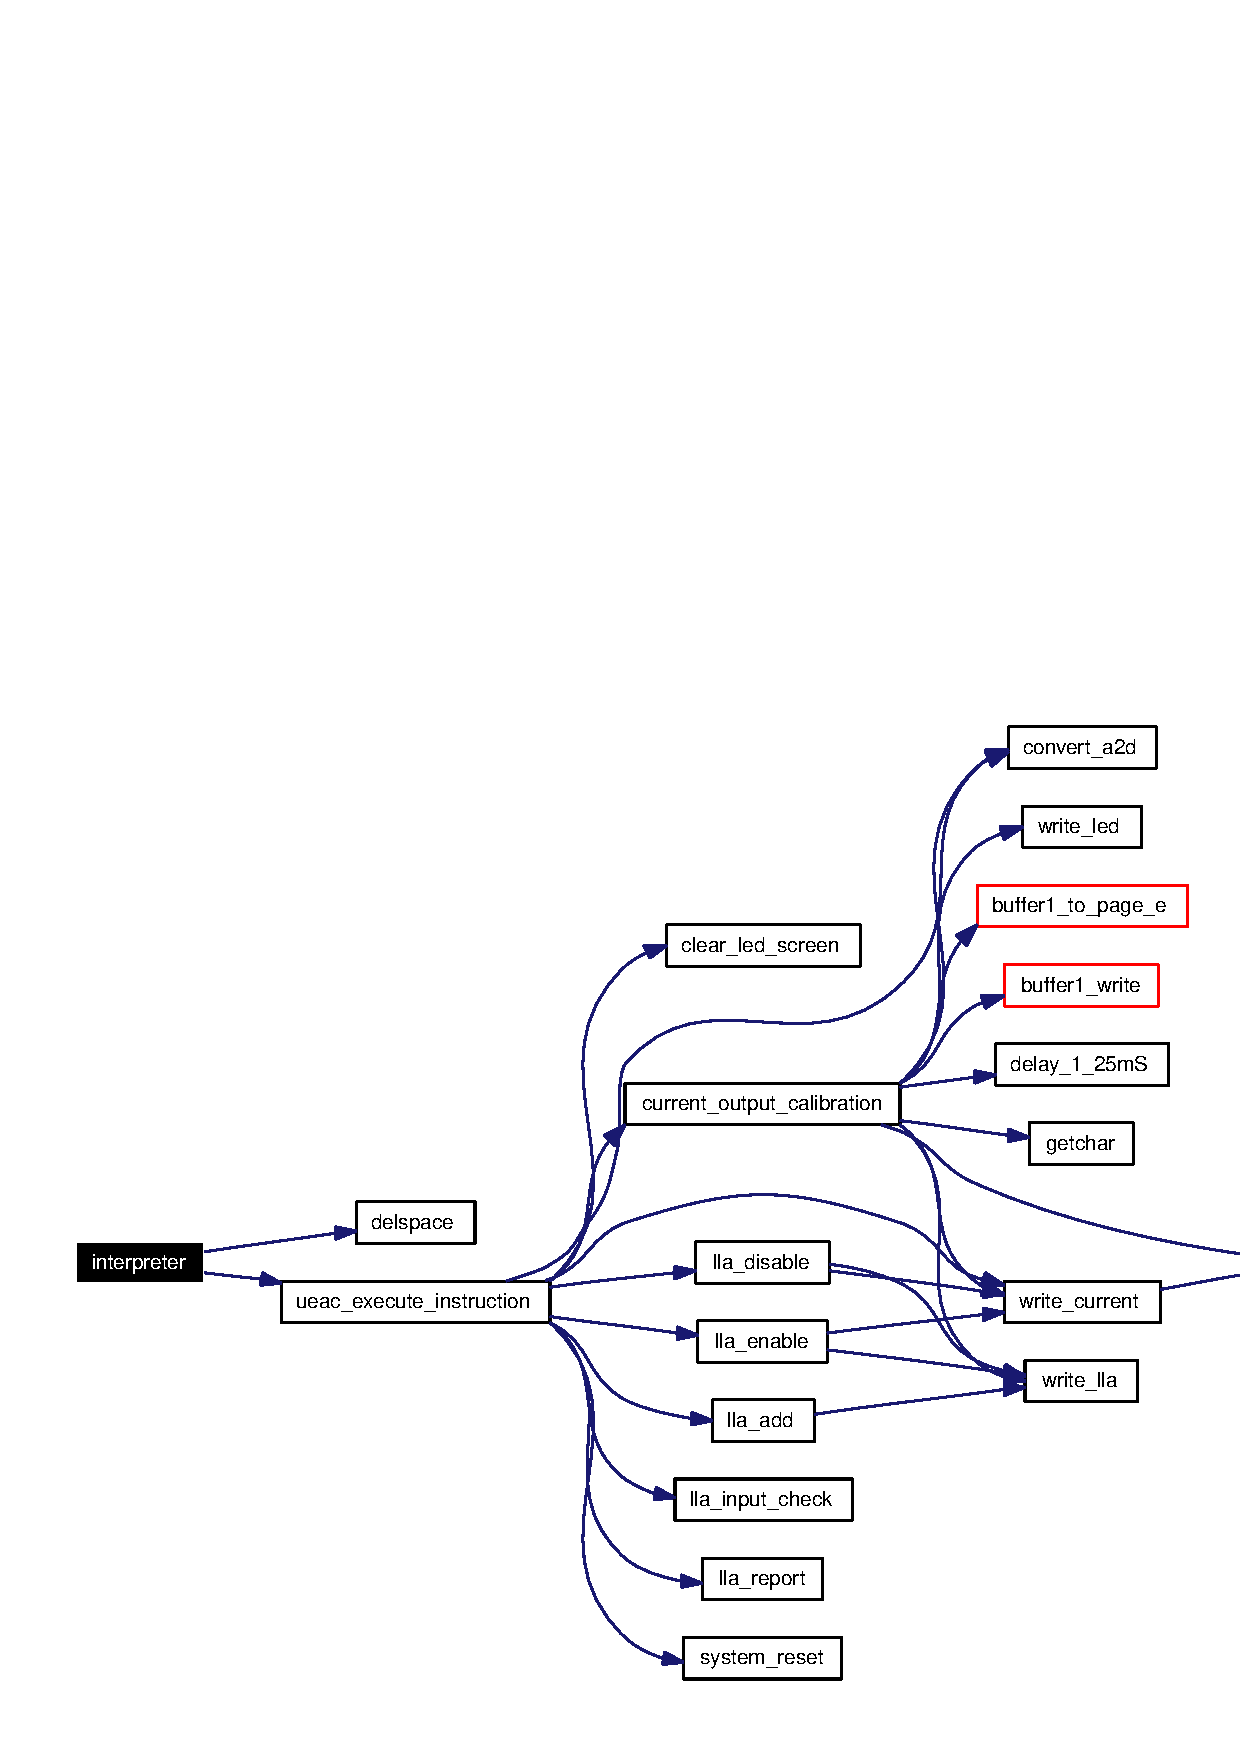
\includegraphics[width=333pt]{interpreter_8c_a9_cgraph}
\end{center}
\end{figure}


\subsection{Variable Documentation}
\index{interpreter.c@{interpreter.c}!CAL@{CAL}}
\index{CAL@{CAL}!interpreter.c@{interpreter.c}}
\subsubsection{\setlength{\rightskip}{0pt plus 5cm}const char {\bf CAL}[$\,$] = \char`\"{}CAL$\backslash$n\char`\"{}}\label{interpreter_8c_a3}




Definition at line 60 of file interpreter.c.

Referenced by interpreter().\index{interpreter.c@{interpreter.c}!DELIMITER@{DELIMITER}}
\index{DELIMITER@{DELIMITER}!interpreter.c@{interpreter.c}}
\subsubsection{\setlength{\rightskip}{0pt plus 5cm}const char {\bf DELIMITER}[$\,$] = \char`\"{},\char`\"{}}\label{interpreter_8c_a0}




Definition at line 57 of file interpreter.c.

Referenced by interpreter().\index{interpreter.c@{interpreter.c}!GRID_NUM_MAX@{GRID\_\-NUM\_\-MAX}}
\index{GRID_NUM_MAX@{GRID\_\-NUM\_\-MAX}!interpreter.c@{interpreter.c}}
\subsubsection{\setlength{\rightskip}{0pt plus 5cm}const char {\bf GRID\_\-NUM\_\-MAX}[$\,$] = \char`\"{}5\char`\"{}}\label{interpreter_8c_a7}




Definition at line 64 of file interpreter.c.\index{interpreter.c@{interpreter.c}!GRID_NUM_MIN@{GRID\_\-NUM\_\-MIN}}
\index{GRID_NUM_MIN@{GRID\_\-NUM\_\-MIN}!interpreter.c@{interpreter.c}}
\subsubsection{\setlength{\rightskip}{0pt plus 5cm}const char {\bf GRID\_\-NUM\_\-MIN}[$\,$] = \char`\"{}1\char`\"{}}\label{interpreter_8c_a6}




Definition at line 63 of file interpreter.c.\index{interpreter.c@{interpreter.c}!LOF@{LOF}}
\index{LOF@{LOF}!interpreter.c@{interpreter.c}}
\subsubsection{\setlength{\rightskip}{0pt plus 5cm}const char {\bf LOF}[$\,$] = \char`\"{}LOF$\backslash$n\char`\"{}}\label{interpreter_8c_a5}




Definition at line 62 of file interpreter.c.

Referenced by interpreter().\index{interpreter.c@{interpreter.c}!LON@{LON}}
\index{LON@{LON}!interpreter.c@{interpreter.c}}
\subsubsection{\setlength{\rightskip}{0pt plus 5cm}const char {\bf LON}[$\,$] = \char`\"{}LON$\backslash$n\char`\"{}}\label{interpreter_8c_a4}




Definition at line 61 of file interpreter.c.

Referenced by interpreter().\index{interpreter.c@{interpreter.c}!RST@{RST}}
\index{RST@{RST}!interpreter.c@{interpreter.c}}
\subsubsection{\setlength{\rightskip}{0pt plus 5cm}const char {\bf RST}[$\,$] = \char`\"{}RST$\backslash$n\char`\"{}}\label{interpreter_8c_a2}




Definition at line 59 of file interpreter.c.

Referenced by interpreter().\index{interpreter.c@{interpreter.c}!TERMINATOR@{TERMINATOR}}
\index{TERMINATOR@{TERMINATOR}!interpreter.c@{interpreter.c}}
\subsubsection{\setlength{\rightskip}{0pt plus 5cm}const char {\bf TERMINATOR}[$\,$] = \char`\"{}$\backslash$n\char`\"{}}\label{interpreter_8c_a1}




Definition at line 58 of file interpreter.c.

Referenced by interpreter().